\documentclass[english,a4paper,12pt]{article}
\usepackage{fancyhdr}
\usepackage{comment}
\usepackage{iftex}
\usepackage{geometry}
\usepackage{booktabs}
\usepackage{enumerate}
\usepackage{amsfonts}
\include{amsmath}
\usepackage{hyperref}
\hypersetup{
    colorlinks=true,
    linkcolor=blue,
    filecolor=magenta,      
    urlcolor=blue,
}
\urlstyle{same}

\newcommand{\tabitem}{~~\llap{\textbullet}~~}
\usepackage{minted}
\usepackage{listings}
\usepackage{graphicx}
\usepackage{caption}
\usepackage{subcaption}
\usepackage{xcolor}
\definecolor{codegreen}{rgb}{0,0.6,0}
\definecolor{codegray}{rgb}{0.5,0.5,0.5}
\definecolor{codepurple}{rgb}{0.58,0,0.82}
\definecolor{backcolour}{rgb}{0.95,0.95,0.92}
%Code listing style named "mystyle"
\lstdefinestyle{mystyle}{
  backgroundcolor=\color{backcolour},   commentstyle=\color{codegreen},
  keywordstyle=\color{magenta},
  numberstyle=\tiny\color{codegray},
  stringstyle=\color{codepurple},
  basicstyle=\ttfamily\footnotesize,
  breakatwhitespace=false,         
  breaklines=true,                 
  captionpos=b,                    
  keepspaces=true,                 
  numbers=left,                    
  numbersep=5pt,                  
  showspaces=false,                
  showstringspaces=false,
  showtabs=false,                  
  tabsize=2
}

%"mystyle" code listing set
\lstset{style=mystyle}
\geometry{verbose,tmargin=4cm,bmargin=3cm,lmargin=1.8cm,rmargin=1.5cm,headheight=2.7cm,headsep=1cm,footskip=3cm}
\usepackage{array}
%
\def \hsp {\hspace{3mm}}
%
\makeatletter
\providecommand{\tabularnewline}{\\}
\makeatother
%
\ifxetex
\usepackage[T1]{fontenc}
\usepackage{fontspec}
\newfontfamily\nakulafont[AutoFakeBold=2]{Nakula}
\newfontfamily\liberationfont{Liberation Sans Narrow}
\newfontfamily\liberationsansfont{Liberation Sans}
\fi
%
\usepackage{tikz}
\usepackage{xcolor}
%
% 
\definecolor{circleorange}{rgb}{1,0.17,0.08}
\definecolor{darkorange}{rgb}{1,0.27,0.1}
\definecolor{orange2}{rgb}{1,0.5,0.15}
\definecolor{orange3}{rgb}{1,0.65,0.25}
\definecolor{yellow1}{rgb}{0.95,0.77,0.2}
\newcommand{\Omit}[1]{}
\fancypagestyle{plain}{
  \fancyhead[LO]
  {
\textbf{Akash Tadwai \\ Vinta Reethu } \newline 
Indian Institute of Technology Hyderabad \newline
Assignment-I \newline
	  }
	  
%
	  \fancyhf[ROH]{

\begin{tikzpicture}[scale=0.25,every node/.style={transform shape}]
\draw [fill=circleorange,circleorange] (5,10) circle (1.15); 
\fill [darkorange] (5.06,8) -- (5.06,2) -- (7.3,1.2) -- (7.3,8.8) -- (5.06,8);
\fill [darkorange] (4.94,8) -- (4.94,2) -- (2.7,1.2) -- (2.7,8.8) -- (4.94,8);
\fill [orange2]    (7.4,8.4) -- (7.4,1.6) -- (8.2,1.2) -- (8.2,8.8) -- (7.4,8.4);
\fill [orange2]    (2.6,8.4) -- (2.6,1.6) -- (1.8,1.2) -- (1.8,8.8) -- (2.6,8.4);
\fill [orange3]    (8.3,8.4) -- (8.3,1.6) -- (9.0,1.2) -- (9.0,8.8) -- (8.3,8.4);
\fill [orange3]    (1.7,8.4) -- (1.7,1.6) -- (1.0,1.2) -- (1.0,8.8) -- (1.7,8.4);
\fill [yellow1]    (9.1,8.4) -- (9.1,1.6) -- (9.7,1.2) -- (9.7,8.8) -- (9.1,8.4);
\fill [yellow1]    (0.9,8.4) -- (0.9,1.6) -- (0.3,1.2) -- (0.3,8.8) -- (0.9,8.4);
\ifxetex
\node [scale=2.1] at (5,-0.1)  {   {\bf {\nakulafont  भारतीय प्रौद्योगिकी संस्थान हैदराबाद }} };
\node [scale=1.8] at (5,-1.2) {   {\bf {\liberationsansfont Indian Institute of Technology Hyderabad}} };
\fi
\end{tikzpicture}
		  }
%
\renewcommand\headrule
 {

\begin{tikzpicture}
\definecolor{yellow1}{rgb}{0.95,0.77,0.2}
\draw[line width=0.75mm, yellow1] (0,0) -- (\textwidth,0);
\end{tikzpicture} 
 }
}
\pagestyle{plain}

\usepackage{blindtext}
\usepackage{amsmath,bm}
\title{\textbf{\underline{\Huge{Assignment-I }}}}
\author{Akash Tadwai - ES18BTECH11019 \\ Vinta Reethu - ES18BTECH11028 \\
}
\date{\today}
\begin{document}
\maketitle
\begin{enumerate}
   \item[\textbf{1.}] { \begin{center}
       \large{\textbf{Linear Regression}}  \\~\\
   \end{center}
   Consider a linear model of the form
$$
y(x, w)=w_{0}+\sum_{d=1}^{D} w_{d} x_{d}
$$
together with a sum-of-squares error function of the form,  
$$ E_{D}(\boldsymbol{w})=\frac{1}{2} \sum_{n=1}^{N}\left\{y\left(\boldsymbol{x}_{n}, \boldsymbol{w}\right)-t_{n}\right\}^2 $$
Now suppose that Gaussian noise $\epsilon_{n}$ with zero mean and variance $\sigma^{2}$ is added independently to each of the input variables $x_{i} .$That
is, independent noise is added to each dimension of the input. By making use of

$$
 \mathbb{E}\left[\epsilon_{n}\right]=0 \ and \quad \mathbb{E}\left[\epsilon_{i} \epsilon_{j}\right]=\delta_{ij}\sigma^2
$$
Show that minimizing $E_{D}(w)$ averaged over the noise distribution is equivalent to minimizing the sum-of-squares error for noise-free input variables with the addition of a weight-decay $\left(L_{2}\right.$ norm $)$ regularization term, in which the bias parameter $w_{0}$ is omitted from the regularizer.} \newline

\textbf{A:} 
Given in the question a Gaussian noise is added to input variables X in all the dimension. After adding this noise out model becomes,

    $$
\begin{aligned}
y^{\prime}\left(x_{i}, w\right) &=w_{0}+\sum_{d=1}^{D} w_{d}\left(x_{id}+\epsilon_{i d}\right) \\
&=w_{0}+\sum_{d=1}^{D} w_{d} x_{i d}+\sum_{d=1}^{D} w_{d} \epsilon_{i d} \\
&=y\left(x_{i}, w\right)+\sum_{d=1}^{D} w_{d} \epsilon_{i d}
\end{aligned}
$$
So our new error function is
$$
\begin{aligned}
E_{D}^{\prime}(w) &=\frac{1}{2} \sum_{n=1}^{N}\left\{y^{\prime}\left(x_{n}, w\right)-t_{n}\right\}^{2} \\
&=\frac{1}{2} \sum_{n=1}^{N}\left\{y\left(x_{n}, w\right)+\sum_{d=1}^{D} w_{d} \epsilon_{n d}-t_{n}\right\}^2 \\
&=\frac{1}{2} \sum_{n=1}^{N}\left\{\left(y\left(x_{n}, w\right)-t_{n}\right)^{2}+2\left(y\left(x_{n}, w\right)-t_{n}\right)\left(\sum_{d=1}^{D} w_{d} \epsilon_{n d}\right)+\left(\sum_{d=1}^{D} w_{d} \epsilon_{n d}\right)^{2}\right\} \\
\end{aligned}
$$
Now we apply expectation on both sides. After using the \textit{\textbf{linearity of expectation}}, we get, \\
$$
\begin{aligned}
\mathbb{E}\left[E_{D}^{\prime}(w)\right]=\frac{1}{2} \sum_{n=1}^{N}\left\{\left(y\left(x_{n}, w\right)-t_{n}\right)^{2}+2\left(y\left(x_{n}, w\right)-t_{n}\right)\left(\sum_{d=1}^{D} w_{d} \mathbb{E}\left[\epsilon_{n d}\right]\right)+\mathbb{E}\left[\left(\sum_{d=1}^{D} w_{d} \epsilon_{n d}\right)^{2}\right]\right\}
\end{aligned}
$$
Given in the question that the mean of noise is 0.
$As \ \mathrm{E}\left[\epsilon_{n d}\right]$ is $0,$ the second term in the above equation is cancelled out.
\\Let us simplify the third term is,
$$
\begin{aligned}
\mathbb{E}\left[\left(\sum_{d=1}^{D} w_{d} \epsilon_{n d}\right)^{2}\right] &=\mathbb{E}\left[\sum_{d=1}^{D} \sum_{d^{\prime}=1}^{D} w_{d} w_{d^{\prime}} \epsilon_{n d} \epsilon_{n d^{\prime}}\right] \\
&=\sum_{d=1}^{D} \sum_{d^{\prime}=1}^{D} w_{d} w_{d^{\prime}} \mathbb{E}\left[\epsilon_{n d} \epsilon_{n d^{\prime}}\right] \\
&=\sum_{d=1}^{D} \sum_{d^{\prime}=1}^{D} w_{d} w_{d^{\prime}} \delta_{d d^{\prime}}\sigma^2 \\
&=\sigma^2\sum_{d=1}^{D} w_{d}^{2}
\end{aligned}
$$
Using these results, we get
$$
\begin{aligned}
\mathbb{E}\left[E_{D}^{\prime}(w)\right] &=\frac{1}{2} \sum_{n=1}^{N}\left\{\left(y\left(x_{n}, w\right)-t_{n}\right)^{2}+\sigma^2\sum_{d=1}^{D} w_{d}^{2}\right\} \\
&=E_{D}(w)+\frac{N}{2}\sigma^2 \sum_{d=1}^{D} w_{d}^{2} 
\end{aligned}
$$
From the above equation we observe that we got a $L_{2}$ regularization term without the bias parameter $w_{0},$.
\newpage
\item[\textbf{2.}] {\begin{center}
       \large{\textbf{Multi-Output Regression}}  \\~\\
   \end{center}
Consider the problem where inputs are associated with multiple real valued outputs $(\mathrm{K}>$
\textbf{1)} known as multi output regression (For e.g. predicting student score across different courses).
$$
\mathbf{y}\left(\mathbf{x}, \mathbf{w}\right)=\mathbf{W}^{\mathrm{T}} \boldsymbol{\phi}(\mathbf{x})
$$
here $y$ is a K-dimensional column vector, $W$ is an $M^{\star}$ K matrix of parameters,and $\boldsymbol{\varphi(x)}$ is an M-dimensional column vector with elements $\varphi_\mathrm{j}(\mathrm{x}),$ with $\varphi_0(\mathrm{x})=1$. \\~\\
\textbf{1.} Provide the expression for the likelihood, and derive $\mathrm{ML}$ and MAP estimates of $\mathrm{W}$ in
the multi output regression case.
}\\
\textbf{A:}
Assuming multiple independent outputs we can model this regression as,\\
$$p(\mathbf{y} \mid \mathbf{x}, \mathbf{W})=\prod_{j=1}^{K} \mathcal{N}\left(y_{j} \mid \mathbf{w}_{j}^{T} \mathbf{x}_{i}, \sigma_{j}^{2}\right)$$
    \begin{itemize}
        \item \textbf{MLE}\\~\\
        The distribution of one of the component of y is given by, 
$$
y_{ij} \sim \mathcal{N}\left(\mathbf{w}_{j}^{T} \mathbf{x}_{i}, {\beta_j}^{-1}\right)
$$
where $i \rightarrow$ 1 to M and $j \rightarrow$ from 1 to K\\
The likelihood of one of the component of y is given by,\\
$$
p(\mathbf{Y}_{j} \mid \mathbf{X}, \mathbf{w}_{j}, \beta_{j})=\prod_{i=1}^{M} \mathcal{N}\left(\mathbf{w}_{j}^{T} \mathbf{x}_{i}, \beta_{j}^{-1}\right)
$$
Taking logarithm on both sides and expanding we get,
$$
\ln p(\mathbf{Y_j} \mid \mathbf{X}, \mathbf{w_j}, \beta_{j})=\sum_{i=1}^{M} \ln \mathcal{N}\left(\mathbf{w_j}^{T} \mathbf{x}_{i}, {\beta_j}^{-1}\right)
$$
Using the density function of a uni variate Gaussian we get,
$$
\begin{aligned}
\ln p(\mathbf{{Y}_{j}} \mid \mathbf{X}, \mathbf{{w}_{j}}, \beta_{j}) &=\sum_{i=1}^{M} \ln \frac{1}{\sqrt{2 \pi \beta_{j}^{-1}}} e^{-\left(y_{ij}-\mathbf{w}_{j}^{T} \mathbf{x}_{i}\right)^{2} / 2 \beta_{j}^{-1}} \\
&=\frac{M}{2} \ln \beta_{j}-\frac{M}{2} \ln(2 \pi)-\frac{\beta_{j}}{2} \sum_{i=1}^{M}\left(y_{ij}-\mathbf{w_j}^{T} \mathbf{x}_{i}\right)^{2}
\end{aligned}
$$
Notice that this is a quadratic function in $\mathbf{w_j},$ which means that we can solve for it by taking the derivative with respect to $\mathbf{w_j},$ setting that expression to $0,$ and solving for $\mathbf{w_j}$ :
\newpage
$$
\begin{aligned}
\frac{\partial \ln p(\mathbf{Y_{j}} \mid \mathbf{X}, \mathbf{w_{j}}, \beta_{j})}{\partial \mathbf{w_{j}}}=\beta_{j} \sum_{i=1}^{M}\left(y_{ij}-\mathbf{w_{j}}^{T} \mathbf{x}_{i}\right) \mathbf{x}_{i}^{T}\\
\end{aligned}
$$
$$
\begin{aligned}
0&=\beta_{j} \sum_{i=1}^{M}\left(y_{ij}-\mathbf{w_{j}}^{T} \mathbf{x}_{i}\right) \mathbf{x}_{i}^{T}\\
0&=\sum_{i=1}^{M} {y_{ij}} \mathbf{x}_{i}^{T}-\mathbf{w_j}^{T} \sum_{i=1}^{M} \mathbf{x}_{i} \mathbf{x}_{i}^{T}
\end{aligned}
$$
Solving for $w_j$ we get
$$
{\hat{\mathbf{w_{j}}}}=\left(\mathbf{X}^{T} \mathbf{X}\right)^{-1} \mathbf{X}^{T} \mathbf{Y_j}
$$

We know that the likelihood factorizes across dimensions, the same does MLE.
$$
\begin{aligned}
{\hat{\mathbf{W}}}=[\hat w_{1},\hat w_{2},.....,\hat w_{M}]
\end{aligned}
$$
where $\boldsymbol{\hat w_{j}}$ is derived above.\\
\item \textbf{MAP}\\~\\
Assuming the Normal Prior with mean 0 and variance $\boldsymbol{S}_{0}^{-1}$, we get,
$$
\mathbf{w_{j}} \sim \mathcal{N}\left(0, \boldsymbol{S}_{0}^{-1} \mathbf{I}\right)
$$
$$
p(\mathbf{Y}_{j} \mid \mathbf{X}, \mathbf{w}_{j}, \beta_{j})=\prod_{i=1}^{M} \mathcal{N}\left(\mathbf{w}_{j}^{T} \mathbf{x}_{i}, \beta_{j}^{-1}\right)
$$
By Bayes' theorem, posterior can be written as
$$
\underbrace{p(\mathbf{w_j} \mid \mathbf{X}, \mathbf{Y_j}, \beta_j)}_{\text {posterior }} \propto \underbrace{p(\mathbf{Y_j} \mid \mathbf{X}, \mathbf{w_j}, \beta_j)}_{\text {likelihood }} \underbrace{p(\mathbf{w_j})}_{\text {prior }}
$$
We now wish to find the value of $\mathbf{w_j}$ that maximizes the posterior distribution. We can maximize the log of the posterior with respect to w  
$$
\ln p(\mathbf{w_j} \mid \mathbf{X}, \mathbf{Y_j}, \beta_j) \propto \ln p(\mathbf{Y_j} \mid \mathbf{X}, \mathbf{w_j}, \beta_j)+\ln p(\mathbf{w_j})
$$
From above derivations we already know the value of 
$$
\ln p(\mathbf{Y_j} \mid \mathbf{X}, \mathbf{w_j}, \beta_{j})=\sum_{i=1}^{M} \ln \mathcal{N}\left(\mathbf{w_j}^{T} \mathbf{x}_{i}, {\beta_j}^{-1}\right)
$$
Calculating the value of $\mathbf{\ln p(w_j)}$
$$
\begin{aligned}
\ln p(\mathbf{w_j}) &=\ln \mathcal{N}\left(0, \boldsymbol{S}_{0}^{-1} \mathbf{I}\right) \\
&=\ln \frac{1}{\left(\left|2 \pi \boldsymbol{S}_{0}^{-1} \mathbf{I}\right|\right)^{\frac{1}{2}}} \exp \left\{-\frac{\boldsymbol{S}_{0}}{2} \mathbf{w_j}^{T} \mathbf{w_j}\right\} \\
&=\mathbf{C}-\frac{\boldsymbol{S}_{0}}{2} \mathbf{w_j}^{T} \mathbf{w_j}
\end{aligned}
$$
By taking derivative and solving for $\boldsymbol{ w_{j}}$\\ Finally we get,
$$
\boldsymbol{\hat w_{j}}=\left(\boldsymbol{X}^{\tau} \boldsymbol{X}+\lambda \boldsymbol{M} \boldsymbol{I}\right)^{-1} \boldsymbol{X}^{T} \boldsymbol{Y_j}
$$
where $\lambda = \frac{S_0}{\beta}$\\
We know that the likelihood factorizes across dimensions, the same does MAP.
$$
\begin{aligned}
{\hat{\mathbf{W}}}=[\hat w_{1},\hat w_{2},.....,\hat w_{M}]
\end{aligned}
$$
where $\boldsymbol{\hat w_{j}}$ is derived above.\\~\\
\textbf{2.} Consider a multi-output regression problem where we have multiple independent outputs in linear regression. Let's consider a 2 dimensional output vector $y_{i} \in \mathrm{R}^2$. Suppose we have some binary input data, $\mathrm{x}_{\mathrm{i}} \in\{0,1\}$. The training data is as given in the right side. Let us embed each $x$ into $2 \mathrm{d}$ using the following basis function: \\
$\varphi$ $(0)=(1,0)^{\top}, \varphi(1)=(0,1)^{\top}$. The model becomes $y=W^{\top} \varphi(x)$ where $W=\left[w_{1}, w_{2}\right]$ is a 2
x 2 matrix, with both $w_{1}$ and $w_{2}$ column vectors. Find the MLE for $w_{1}$ and $w_{2}$.\\~\\.
$$
\begin{array}{c|l}
\mathrm{x} & \mathrm{y} \\
\hline 0 & (-1,-1)^{T} \\
0 & (-1,-2)^{T} \\
0 & (-2,-1)^{T} \\
1 & (1,1)^{T} \\
1 & (1,2)^{T} \\
1 & (2,1)^{T}
\end{array}
$$
\textbf{A:}
We know that $$\boldsymbol{Y}=\boldsymbol{W^{T}}\boldsymbol{\varphi(x)}$$
By expanding this we get,
$$
\left(\begin{array}{c}
\hat{\mathbf{y}}_{1} \\
\hat{\mathbf{y}}_{2}
\end{array}\right)=\left(\begin{array}{c}
\hat{\mathbf{w}}_{1}^{T} \\
\hat{\mathbf{w}}_{2}^{T}
\end{array}\right)\left(\begin{array}{l}
\phi_{1}(x) \\
\phi_{2}(x)
\end{array}\right)
$$
Our design matrix $\mathbf{X}$ which is obtained by plugging the values if x in our data set in $\mathbf{\varphi(x)}$\\
$$\mathbf{X}_{1}=\mathbf{X}_{2}=\mathbf{X}=\left(\begin{array}{ll}
1 & 0 \\
1 & 0 \\
1 & 0 \\
0 & 1 \\
0 & 1 \\
0 & 1
\end{array}\right)\\
\mathbf{y}_{1}=\left(\begin{array}{c}
-1 \\
-1 \\
-2 \\
1 \\
1 \\
2
\end{array}\right)\\ \mathbf{y}_{2}=\left(\begin{array}{c}
-1 \\
-2 \\
-1 \\
1 \\
2 \\
1
\end{array}\right)
$$
$$
{\hat{\mathbf{w_{1}}}}=\left(\mathbf{X}^{T} \mathbf{X}\right)^{-1} \mathbf{X}^{T} \mathbf{Y_1}
$$
$$
{\hat{\mathbf{w_{2}}}}=\left(\mathbf{X}^{T} \mathbf{X}\right)^{-1} \mathbf{X}^{T} \mathbf{Y_2}
$$
\newpage
$$
\left(\mathbf{X}^{T} \mathbf{X}\right)^{-1} =\left(\begin{array}{ll}
\frac{1}{3} & 0    \\
0 & \frac{1}{3} \\
\end{array}\right)
$$ \\
$$
\left(\mathbf{X}^{T} \mathbf{X}\right)^{-1} \mathbf{X}^{T}=\left(\begin{array}{llllll}
\frac{1}{3} & \frac{1}{3} & \frac{1}{3} & 0 & 0 & 0 \\
0 & 0 & 0 & \frac{1}{3} & \frac{1}{3} & \frac{1}{3}
\end{array}\right)
$$
By multiplying by $y_{1}$ we get,
$$
\hat{\mathbf{w}}_{1}=\left(\begin{array}{c}
-\frac{4}{3} \\
\frac{4}{3}
\end{array}\right)
$$
By multiplying by $y_{2}$ we get,
$$
\hat{\mathbf{w}}_{2}=\left(\begin{array}{c}
-\frac{4}{3} \\
\frac{4}{3}
\end{array}\right)
$$
Hence our MLE of $\mathbf{W}$ is,
$$
\hat{\mathbf{W}}=\left(\begin{array}{cc}
-\frac{4}{3} & -\frac{4}{3} \\
\frac{4}{3} & \frac{4}{3}
\end{array}\right)
$$
\\
\end{itemize}
\vspace{2cm}
\item[\textbf{3.}]  \begin{center}
       \large{\textbf{ML and MAP estimation of
Poisson Distribution}}\\~\\
   \end{center}
   
\begin{itemize}
    \item \textbf{Derivation of maximum likelihood estimation :} \\\\
Suppose that $X=\left(X_{1}, X_{2}, \ldots, X_{n}\right)$ are iid observations from a Poisson distribution with unknown parameter $\lambda .$ The likelihood function is:
\begin{center}
$$
\begin{aligned}
f\left(x_{i}, \lambda\right)= \frac{e^{-\lambda} \lambda^{x_{i}}}{x_{i} !} \\
L(\lambda, \boldsymbol{x})=\prod_{i=1}^{n} f\left(x_{i}, \lambda\right)=\prod_{i=1}^{n} \frac{e^{-\lambda} \lambda^{x_{i}}}{x_{i} !} &=\frac{e^{-n \lambda} \lambda^{\sum x_{i}}}{\prod_{i=1}^{n} x_{i} !} \\
I(\lambda)=\log L(\lambda, \boldsymbol{x})=-n \lambda+\sum x_{i} \log \lambda-\log \left\{\prod_{i=1}^{n} x_{i} !\right\} \\
\frac{d l}{d \lambda}=-n+\frac{\sum x_{i}}{\lambda}=\frac{\sum x_{i}-n \lambda}{\lambda} &>0 \quad \text { if } \lambda<\bar{x} \\
&<0 \quad \text { if } \lambda>\bar{x}
\end{aligned}
$$
\end{center}

 $\hat{\lambda}_{MLE}=\bar{X}$ is the $\mathrm{MLE}$ of $\lambda$.
 
\newpage

\item \textbf{Derivation of maximum aposteriori estimation:}\\\\
According to Baye's theorem
$$
\mathcal{P}(\lambda \mid x)=\frac{P(x \mid \lambda) \cdot P(\lambda)}{P\left(x\right)},\quad \text{where } P(x) \text{ is independent of } \lambda
$$
We know that
$$
\mathcal{P}(x \mid \lambda)=\prod_{i=1}^{N} \frac{e^{-\lambda}{\lambda}^{x_i}}{{x_{i} !} }
$$
\textbf{Why we chose Gamma Prior?}\\
We chose gamma prior as it is conjugate distribution for poission.\\
Taking Gamma Prior,
$$
P(\lambda)=\frac{\beta^{\alpha} \lambda^{\alpha-1} e^{-\beta \lambda}}{\Gamma(\alpha)}
$$
Now applying Baye's theorem, \\
$$
\begin{aligned}
P(\lambda \mid x) &=\frac{e^{-n \lambda} \lambda^{\sum x_{i}}}{\prod_{i=1}^{N} x_{i} !} \cdot \frac{\lambda^{\alpha-1} \cdot e^{-\beta \lambda}}{\Gamma(\alpha)} \\
&=k \cdot \lambda^{(\sum x_{i}+\alpha-1)} \cdot e^{-\lambda(n+\beta)} \\
\Rightarrow \operatorname{Gamma}(\sum x_{i}+\alpha, \beta+N) \\
\end{aligned}
$$
Hence the MAP estimate would be the mode of the posterior distribution. \\
We know that the Mode of Gamma distribution is, $\frac{\alpha -1}{\beta}$

 $\hat{\lambda}_{MAP}=\frac{\sum x_{i}+\alpha - 1}{N+\beta}$ is the $\mathrm{MAP}$ of $\lambda$.\\

 \end{itemize}
 \textbullet \textbf{Procedure :}
 \begin{itemize}
     \item First we obtained the data from this \href{http://www.randomservices.org/random/data/HorseKicks.txt}{link} using \textbf{wget.}
     \item Using the above mathematical equations we obtained MLE and RMSE.
     \item We have plotted the Number of corp years vs Number of deaths to visualize the data.
     \item Next we obtained MAP estimates by choosing suitable alpha, beta which is further explained in Observations below.
     \item We plotted Likelihood,Prior,Posterior graphs by using the above derived mathematical equations.
 \end{itemize}
 \newpage
 \textbullet \textbf{Plots :}
 \begin{itemize}
     \item \textbf{Final plot of number of deaths by Horsekicks:}
     
     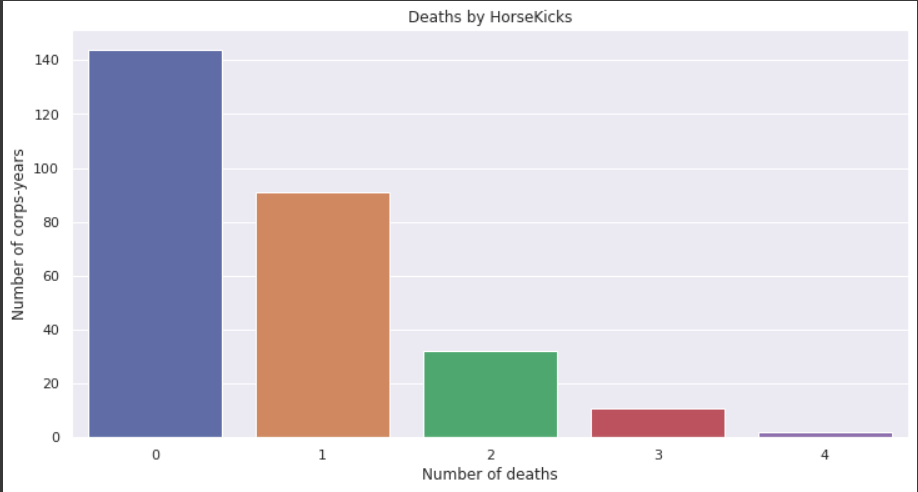
\includegraphics[width=10cm]{pictures/Q3/Observations_Q3_2.png}
     
     \item \textbf{Lambda estimate and RMSE (predictions) for each corp using MLE:}
     
    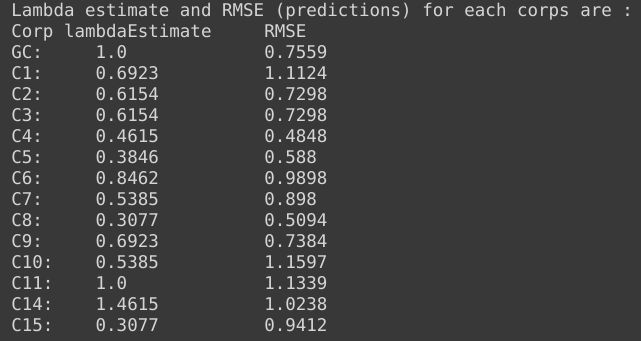
\includegraphics[width=11cm]{pictures/Q3/Observations_Q3_1.png}
     
    \item \textbf{Lambda estimate and RMSE (predictions) for each corp using MAP:}
    
    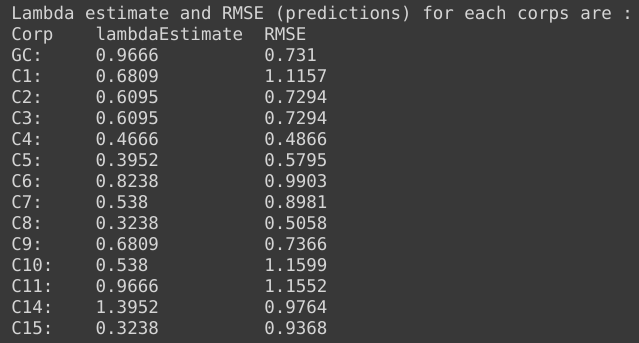
\includegraphics[width=11cm]{pictures/Q3/Observations_Q3_3.png}
    
    \newpage
    \textbf{Likelihood, Prior and Posterior Plots for 2,4,6 corps}
   {\begin{figure} [h!]
     \centering
     \begin{subfigure}[b]{0.3\textwidth}
         \centering
         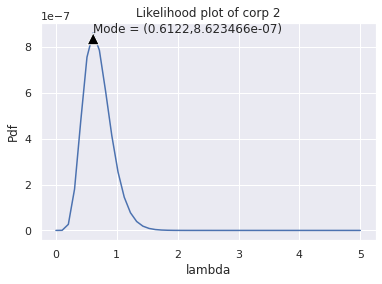
\includegraphics[width=\textwidth]{pictures/Q3/Likelhood_C2.png}
         \caption{$Likelihood$}
         \label{Likelihood}
     \end{subfigure}
     \hfill
     \begin{subfigure}[b]{0.3\textwidth}
         \centering
         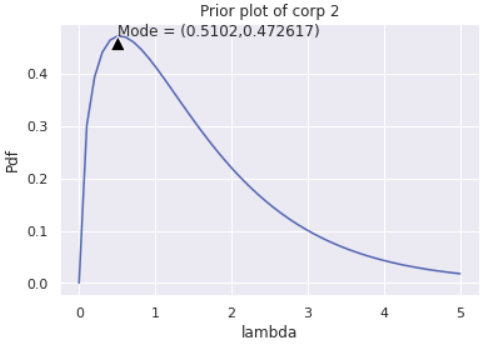
\includegraphics[width=\textwidth]{pictures/Q3/Prior_C2.png}
         \caption{$Prior$}
         \label{Prior}
     \end{subfigure}
     \hfill
     \begin{subfigure}[b]{0.3\textwidth}
         \centering
         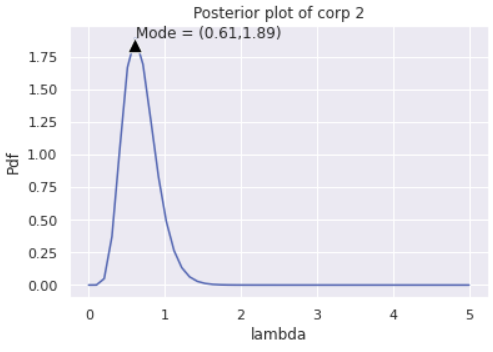
\includegraphics[width=\textwidth]{pictures/Q3/Posterior_C2.png}
         \caption{$Posterior$}
         \label{Posterior}
     \end{subfigure}
        \caption{Corp 2}
        \label{Corp 2 }
\end{figure}}



 {\begin{figure} [h!]
     \centering
     \begin{subfigure}[b]{0.3\textwidth}
         \centering
         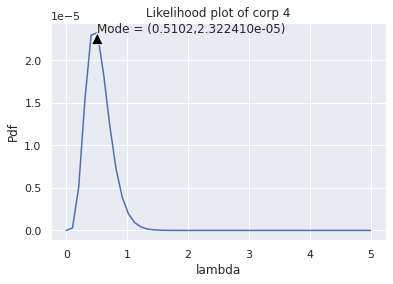
\includegraphics[width=\textwidth]{pictures/Q3/Likelihood_C4.png}
         \caption{$Likelihood$}
         \label{Likelihood}
     \end{subfigure}
     \hfill
     \begin{subfigure}[b]{0.3\textwidth}
         \centering
         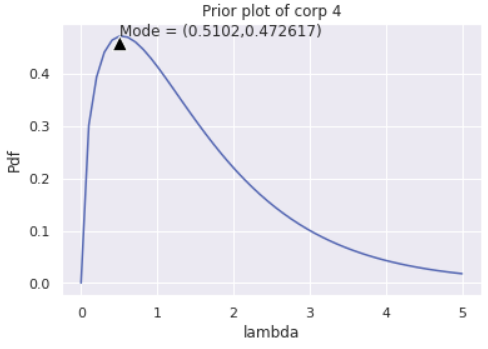
\includegraphics[width=\textwidth]{pictures/Q3/Prior_C4.png}
         \caption{$Prior$}
         \label{Prior}
     \end{subfigure}
     \hfill
     \begin{subfigure}[b]{0.3\textwidth}
         \centering
         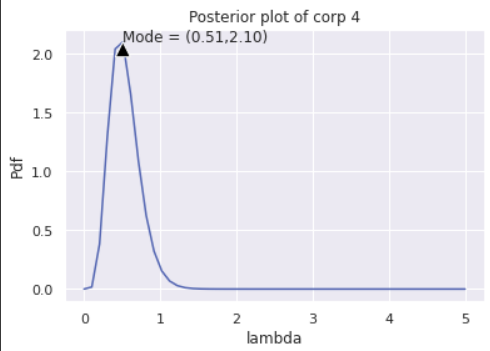
\includegraphics[width=\textwidth]{pictures/Q3/Posterior_C4.png}
         \caption{$Posterior$}
         \label{Posterior}
     \end{subfigure}
     \caption{Corp 4}
        \label{Corp 4 }
\end{figure}}

 {\begin{figure}[h!]
     \centering
     \begin{subfigure}[b]{0.3\textwidth}
         \centering
         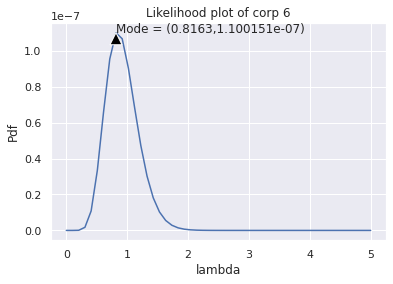
\includegraphics[width=\textwidth]{pictures/Q3/Likelihood_C6.png}
         \caption{$Likelihood$}
         \label{Likelihood}
     \end{subfigure}
     \hfill
     \begin{subfigure}[b]{0.3\textwidth}
         \centering
         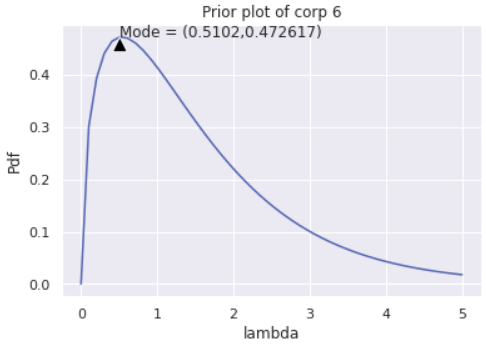
\includegraphics[width=\textwidth]{pictures/Q3/Prior_C6.png}
         \caption{$Prior$}
         \label{Prior}
     \end{subfigure}
     \hfill
     \begin{subfigure}[b]{0.3\textwidth}
         \centering
         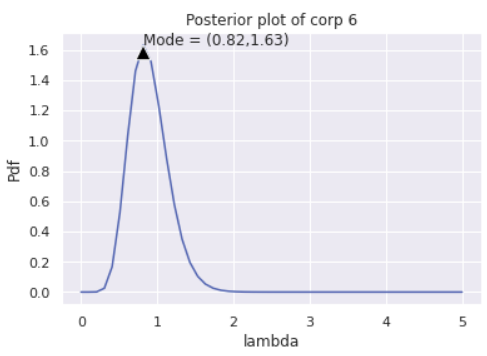
\includegraphics[width=\textwidth]{pictures/Q3/Posterior_C6.png}
         \caption{$Posterior$}
         \label{Posterior}
     \end{subfigure}
        \caption{Corp 6}
        \label{Corp 4 }
\end{figure}}
 \end{itemize}
 \newpage
 
\textbullet\textbf{Observations:}
    \begin{itemize}
        \item As Gamma distribution is the prior for Poisson distribution. We chose $\alpha$ and $\beta$ such that, Mode of the prior is tending to zero, as parameters estimated using MLE are close to zero. As some of the lambdas are also tending to 1 we choose the Gamma distribution such that the Variance is maximum possible.
      \begin{equation} \label{eq1}
\begin{split}
Mode &\rightarrow   max(0,\frac{\alpha -1}{\beta }) \\
Variance &\rightarrow \frac{\alpha}{\beta ^ 2}\\
\end{split}
\end{equation}
After clear examination of the effect of different alpha,betas on training data,\\we chose:
$\alpha \rightarrow 1.5325$,
$\beta \rightarrow 1$
\vspace{2cm}
\item \textbf{Mode of distributions :}\\
We plotted Likelihood, Prior, Posterior plots for the following corps and used the graph to obtain the mode of distributions. We can see from the graphs that posterior density graph has density \textbf{somewhere between} prior and likelihood densities.
We know that mode means the maximum number in the given set of observations, In our case mode of distribution gives the lambda for which we have the highest probability density. Among 2,4,6 corps \textit{Corp 6 has the highest posterior Lambda} and hence are more likely to be dead by HorseKicks.
    \begin{itemize}
        \item \textbf{Corp 2:}\\
    Likelihood : [0.6122449, 8.623466e-07]\\
    Prior : [0.5102, 0.472617] \\
    Posterior : [0.61, 1.89]
    \item \textbf{Corp 4:}\\
    Likelihood : [0.51020408, 2.322410e-05]\\
    Prior : [0.5102, 0.472617]\\
    Posterior : [0.51, 2.10]
    \item \textbf{Corp 6:}\\
    Likelihood : [0.81632653, 1.100151e-07]\\
    Prior : [0.5102, 0.472617]\\
    Posterior : [0.82, 1.63]
    \end{itemize}
    \end{itemize}
    
    
\newpage

\item[\textbf{4.}]  \begin{center}
       \large{\textbf{Bike Sharing Demand}}\\~\\
   \end{center}
   \begin{itemize}
        \item \textbf{Mean :}\\\\
       If $\mathbf{x} \in \mathbb{R}^{n}$ is a vector of independent variables, We know that Poisson regression model takes the form,
$$
\log (\mathrm{E}(Y \mid \mathbf{x}))=\alpha+\beta^{T} \mathbf{x}
$$
where $\alpha \in \mathbb{R}$ and $\beta \in \mathbb{R}^{n}$.

Given a Poisson regression model $\theta$ and an input vector $x,$ the predicted mean of Poisson distribution is given by
$$
\mathrm{E}(Y \mid \mathbf{x})=e^{\theta^{T} \mathbf{x}}
$$  
\item \textbf{Maximum likelihood estimation in Poisson regression :}\\\\

Given a set of parameters $\theta$ and an input vector $x$, the mean of the Poisson distribution, is given by
$$
\lambda=\mathrm{E}(Y \mid x)=e^{\theta^{T} x}
$$
and thus, the Poisson probability mass function is given by
$$
p(y \mid x ; \theta)=\frac{\lambda^{y}}{y !} e^{-\lambda}=\frac{e^{y \theta^{T} x} e^{-e^{\theta^{T} x}}}{y !} 
$$
Now suppose we are given a data set consisting of $m$ vectors $x_{i} \in \mathbb{R}^{n+1}, i=1, \ldots, m$, along with a set of $m$ values $y_{1}, \ldots, y_{m} \in \mathbb{N}$. Then, for a given set of parameters $\theta$, the probability of attaining this particular set of data is given by
$$
p\left(y_{1}, \ldots, y_{m} \mid x_{1}, \ldots, x_{m} ; \theta\right)=\prod_{i=1}^{m} \frac{e^{y_{i} \theta^{T} x_{i}} e^{-e^{\theta^{T} x_{i}}}}{y_{i} !}
$$
By the method of maximum likelihood, we want to find the set of parameters $\theta$ that makes this probability as large as possible. 
$$
L(\theta \mid X, Y)=\prod_{i=1}^{m} \frac{e^{y_{i} \theta^{T} x_{i}} e^{-e^{\theta^{T} x_{i}}}}{y_{i} !}
$$
Now we take the log on both sides of Likelihood function:
$$
\ell(\theta \mid X, Y)=\log L(\theta \mid X, Y)=\sum_{i=1}^{m}\left(y_{i} \theta^{T} x_{i}-e^{\theta^{T} x_{i}}-\log \left(y_{i} !\right)\right)
$$
Notice that the parameters $\theta$ only appear in the first two terms of each term in the summation. Therefore, given that we are only interested in finding the best value for $\theta$ we may drop the $y_{i}^{T}$ and simply write
$$
\ell(\theta \mid X, Y)=\sum_{i=1}^{m}\left(y_{i} \theta^{T} x_{i}-e^{\theta^{T} x_{i}}\right)
$$
As we don't get closed form solution we minimise the negative log-likelihood and update the weights.
\item \textbf{Cost function :}\\\\
We take the cost function as the negative log likelihood,
$$J\left(\theta_{0}, \theta_{1}, \theta_{2}, \ldots\right)=-\frac{1}{2m}\sum_{i=1}^{m}\left(y_{i} \theta^{T} x_{i}-e^{\theta^{T} x_{i}}\right)$$

By taking the derivative of loss function, $-\ell(\theta \mid X, Y)$ w.r.t $\theta$,\\ we get,
$$ \nabla \mathrm{E}(\mathbf{w})=\frac{\partial J(\theta \mid X, Y)}{\partial \theta}=-\frac{1}{2m}\sum_{i=1}^{m}\left(y_{i} x_{i}-e^{\theta^{T} x_{i}} x_{i}\right)$$    
Hence the Gradient Descent Update is as follows,
$$w^{n e w}=w -\frac{\eta}{2m} \sum_{i=1}^{m}\left( e^{\theta^{T} x_{i}}  - y_{i} \right) x_{i}  $$  

$\eta:$ Learning Rate
\vspace{2cm}
\item \textbf{Statistics of the dataset :} \\\\
   The mean count per month is 191.14315 \\
The median count per month is 205.29504\\
The mean count per each day of week is 190.69694\\
Standard Deviation of temp is 0.192556\\
Minimum counts in a day is 1.00\\
\newpage
\item \textbf{Plots:}
   \end{itemize} 
   
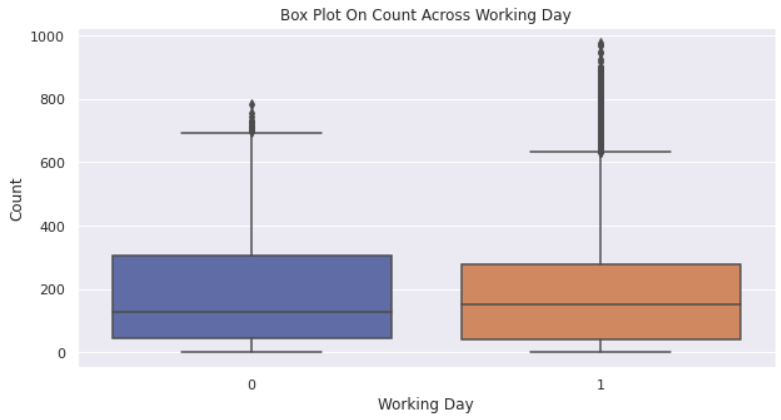
\includegraphics[width=15cm]{pictures/Plot_Q4_1.png} \\ 
\vspace{2cm}
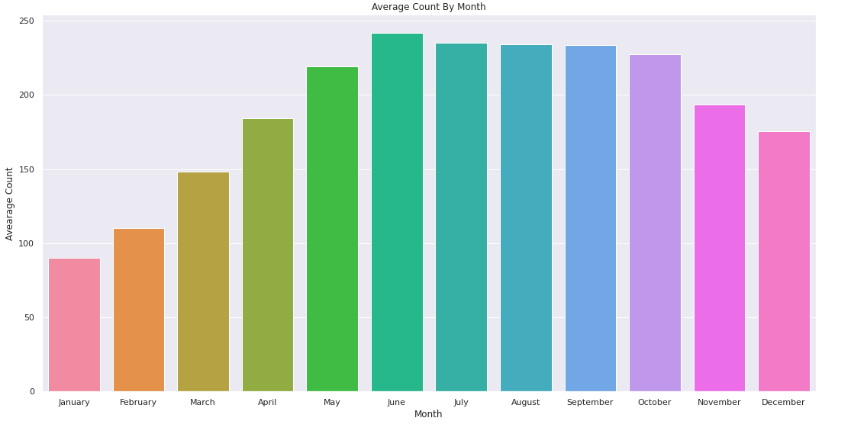
\includegraphics[width=15cm]{pictures/Plot_Q4_2.png} \\ 
\newpage
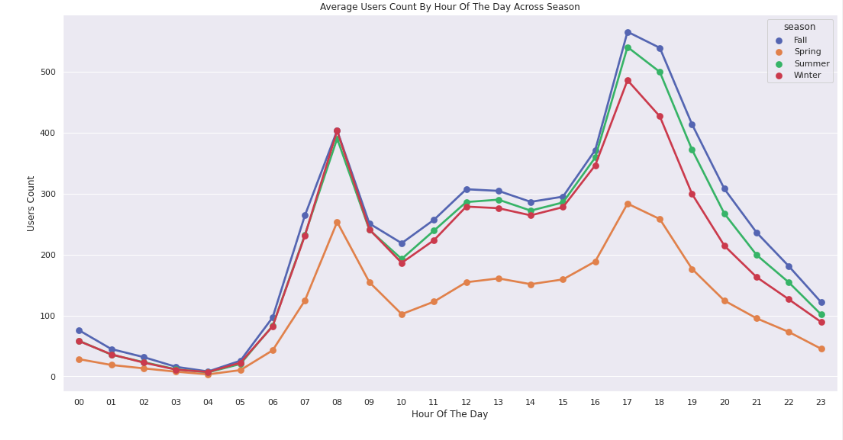
\includegraphics[width=12cm]{pictures/Plot_Q4_3.png} \\ 
\vspace{1cm}
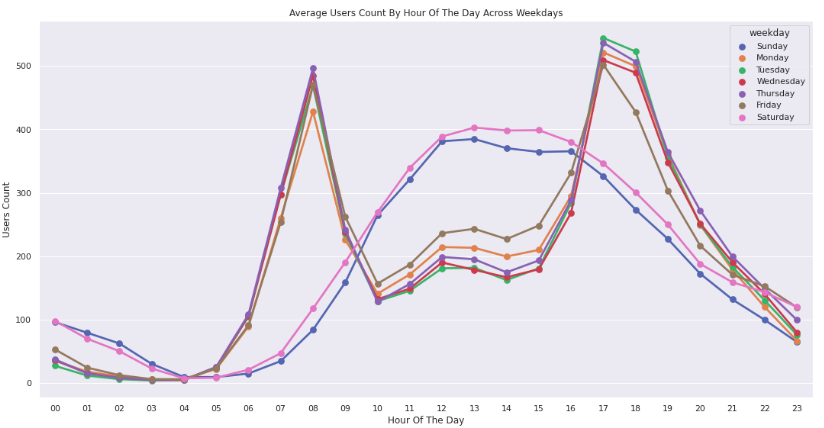
\includegraphics[width=12cm]{pictures/Plot_Q4_4.png} \\
\vspace{1cm}
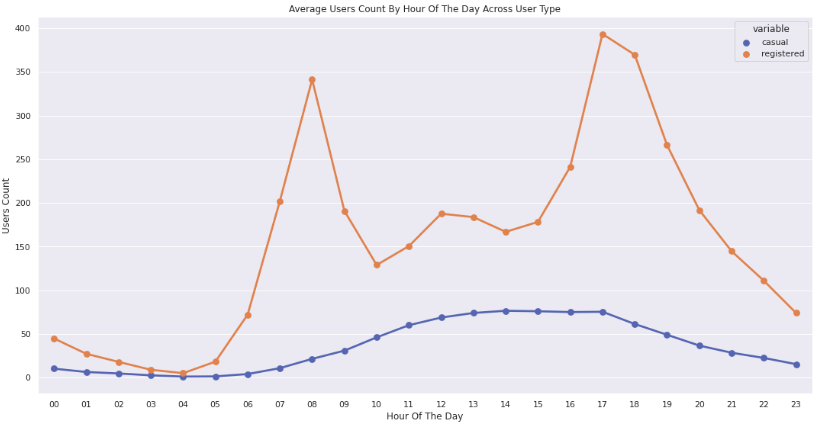
\includegraphics[width=12cm]{pictures/Plot_Q4_5.png} \\

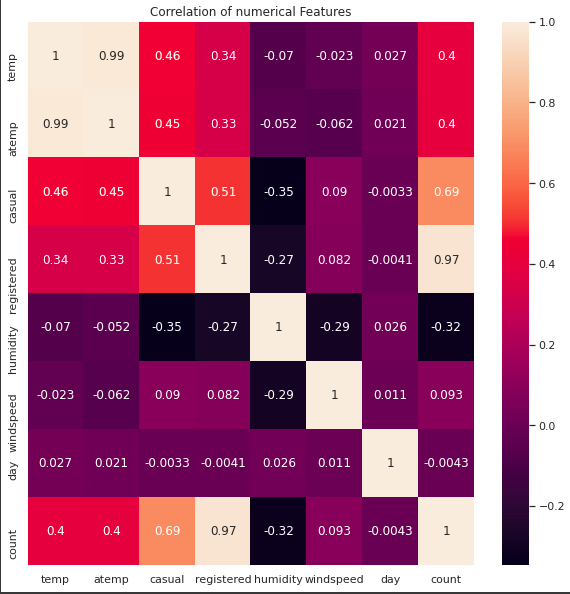
\includegraphics[width=10cm,height=8cm]{pictures/CorrelnPlot_Q4.png} \\\\
\textbullet\textbf{Procedure :}
\begin{itemize}
    \item First we obtained the data from this \href{https://archive.ics.uci.edu/ml/machine-learning-databases/00275/Bike-Sharing-Dataset.zip}{link} using \textbf{wget.}
    \item We used the variables present in the dataset to plot the graphs on training set.
    \item Using the numerical variables we plotted the heat map to see the correlated features. Further explanation of this is given in observation section below.
    \item Next we took the categorical features and did the one hot encoding on those vectors.

\item We know that hour,weekday,season,year,weather,holiday,working day are categorical variables. 
\item So we did one-hot encoding on these variables, We have dropped one of the highly correlated features (eg. temp and atemp)
\item We used Poisson regression to model the count and obtained the hyperparameter by tuning for different values.
\item We have done Poisson regression with and without regularisation and obtained the values, which are given in Observation section below.\\
\end{itemize}
\textbullet\textbf{Observations:}\\
From the correlation plot above we can see that,
\begin{itemize}
    \item Count variable has got little dependency on "temp" and "humidity".
    \item "Casual" and "Registered" features should be dropped since they are just leakage variables.
    \item "atemp" and "temp" are highly correlated and hence one of them is to be dropped.
\end{itemize}
\newpage
\textbullet After applying L1 and L2 norm regularization over weight vectors, and find the best hyper-parameter
settings for the mentioned problem using validation data we obtained :
\begin{itemize}
    \item \textbf{No regularisation :}\\
    RMSE : 108.6739\\
    Learning Rate : 4*1e-3\\
    Iterations : 650
    \item \textbf{L1 Norm :}\\
    RMSE : 108.8211 \\
    Learning Rate : 4.5*1e-3\\
    Iterations : 700\\
    Lambda : 2
    \item\textbf{L2 Norm :} \\
    RMSE : 108.8151 \\
    Learning Rate : 4.5*1e-3\\
    Iterations : 650\\
    Lambda : 0.5
\end{itemize}

\textbullet\textbf{Important Features:}
\begin{itemize}
    \item By inferring from the weights of the model with and without regularisation and the correlation plot we have drawn above,  we see that \textbf{hour of the day, season and humidity} are playing an important role in estimation of Counts in the dataset.
    \item Variables such as \textbf{casual},\textbf{registered} are leaky variables and hence removed while training.
    \item Highly correlated variables are \textbf{temp and atemp} and we removed \textbf{atemp} while training.
\end{itemize}

 {\textbf{Colab Notebook links}}:
\begin{itemize}
    \item \href{https://colab.research.google.com/drive/1RIH4N19g8it21CmKt_tUkKTUPszNoOGc?usp=sharing}{Horse-Kicks}
    \item \href{https://colab.research.google.com/drive/13H5d6ahvjZSX75n3Lm-WQh5V6Pe4IM3P?usp=sharing}{Bike-Sharing}
\end{itemize}


\end{enumerate}
\textbf{Note}: \\ 
This is a \LaTeX Generated document,
whole project can be viewed \href{https://www.overleaf.com/read/vddfhzgctpvn}{here}
\vspace{2cm}
\center ******THE END******
\newpage    
\end{document}